% !TeX root = ../SDonchezThesis.tex

\chapter{Key Aggregate Cryptography}\label{ch:keyAggregateCryptography}
One of the key tenants of the architecture proposed in \cite{bag_cryptographically_2020}, and which is similarly incorporated into this work's architecture, is the use of Key Aggregate Cryptography (KAC) to enable the secure and efficient exchange of encrypted bitstreams between a tenant designer and the CSP. KAC is an asymmetric cryptographic mechanism whereby a single set of public and private ``Master Keys'' can be used in conjunction with a set of ``Aggregate Keys'', each of which affords decryption access to only a subset of the data originally encrypted. In \cite{bag_cryptographically_2020}, the authors utilize this functionality to ensure that only the specific target FPGA can decrypt the tenant bitstream, greatly reducing the scope of vulnerability of the bitstream to third-party compromise.

The concept of Key Aggregation Cryptography is very much a novel area for academic research, having been first proposed in 2013 in \cite{chu_key-aggregate_2014}. The remainder of this chapter will outline the concepts behind KAC based encryption in detail, as well as discuss the use of it in \cite{bag_cryptographically_2020} to facilitate secured bitstream exchange. It will then conclude with the discussion of the cryptosystem within the context of the proposed system architecture, as it relates to the memory isolation functionality discussed in \ref{ch:dmaProtection} as well as with regards to the efficient use of the cryptocore across the various partitions.

\section{Background}\label{sec:KACBackground}
The concept of a Key Aggregate Cryptosystem was first proposed in \cite{chu_key-aggregate_2014} as a means to facilitate the convenient distribution of media assets with targeted access permissions. In today's infrastructure, one could envision its function in a manner similar to Google's Drive storage (or Microsoft's comparable OneDrive). In both instances, a user can upload a set of files, and provide unique permissions on each, thereby enabling only the intended users to access each file. Of course, the technical implementation of these systems does not actually utilize the concept of Key Aggregate Cryptosystems, but the effect is similar.

The implementation of a KAC system is based heavily on ecliptic curve cryptography, a common cryptosystem in widespread use in modern encryption. It is comprised of 5 distinct steps, each of which is discussed below:
\begin{itemize}
    \item \textbf{System Initialization}: The implementer specifies a number of distinct partitions (indices) for the system, as well as a key strength, $\lambda$. $\lambda$ is used to constrain the size of the random data set used to generate the Master Public and Secret Keys, which enable the encryption and decryption of all partitions' data. 
    \item \textbf{Key Generation}: The implemented then specifies (or randomly selects, perhaps programmatically) a random value which is utilized in conjunction with the random dataset (constrained by the $\lambda$ value from the \textit{System Initialization} step) to generate the Master Public and Secret Keys. 
    \item \textbf{Data Encryption}: The data to be encrypted is assigned an index, and is then encrypted using the Master Public Key. The details of the encryption process far exceed the scope of this effort, but generally, given the Master Public Key, the index value, and the data to be encrypted, the engine outputs the ciphertext representative of the data.
    \item \textbf{Partition Key Extraction}: Given a set of indices (which may contain as few as a single index), the extraction functionality generates an Aggregate Secret Key, which is sufficient to decrypt the data associated with the given indices, while not enabling the decryption of any other data. The nature of this process is once again outside the scope of this research effort, but it is important to note that the size of the Aggregate Secret Key is constant, regardless of the number of indices in the set it unlocks.
    \item \textbf{Data Decryption}: Given the Aggregate Secret Key, in conjunction with an index value covered by said key, the decryption process reverses the encryption, yielding the original data. Attempts to decrypt data which is not covered by the Aggregate Secret Key can not only easily be detected, but are mathematically guaranteed to result in a decryption failure.   

\end{itemize}

Figure \ref{fig:KAC_simple} shows a simple example of the KAC process, implemented in the context of encrypting data for shared network storage.

\begin{figure}[ht]
    \centering
    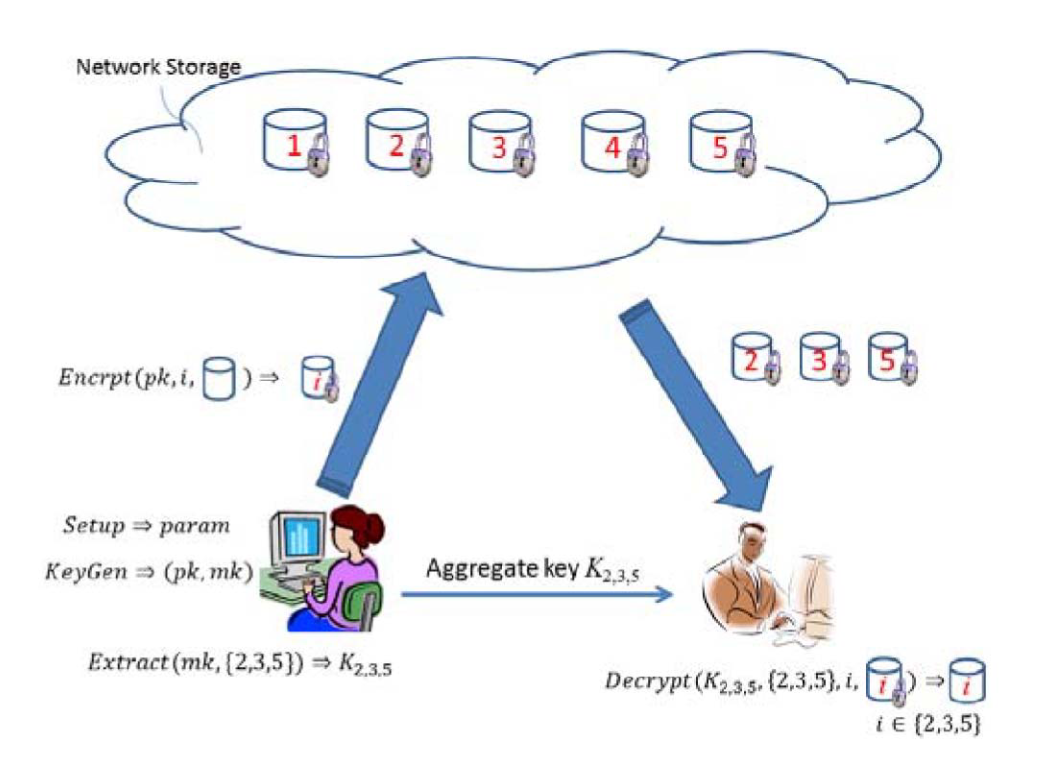
\includegraphics[width=0.7\textwidth]{KAC_simple}
    \caption[KAC Example]{A trivial example of a KAC system in use for network storage. \cite{chu_key-aggregate_2014}}
    \label{fig:KAC_simple}
\end{figure}

An infrastructure such as is afforded by a Key Aggregate Cryptosystem is doubtlessly invaluable for many applications where centralized and easy encryption of data is desired while granularity of access control is still necessary. Although the original developers of the concept in \cite{chu_key-aggregate_2014} present it as a mechanism for facilitating patient access to medical records (and the easy delegation of dependents, etc.), it also has tremendous potential in cloud applications, especially in multi-tenant systems where decryption resources are central and shared. The authors of \cite{bag_cryptographically_2020} implement just such a system in their solution to this design paradigm.

\section{Utilization in Literature}\label{sec:KACLiterature}
The authors of \cite{bag_cryptographically_2020} utilize a hybrid KAC-AES infrastructure to leverage the strengths of both symmetric and asymmetric encryption. KAC, as an ECC derivative, is an asymmetric encryption protocol. Accordingly, different keys are utilized for encryption and decryption operations. This is a tremendous boon from a security perspective in this instance, as the secret key used for decryption need never be provided to tenant designers for encryption. Instead, it can reside in the hardware performing the decryption, likely in isolated memory such as Battery Backed RAM (BBRAM) or Fusible Flash Memory (commonly known as eFUSE in Xilinx devices). In the case of KAC specifically, this strength is enhanced in that the index value must also be known in addition to the secret (aggregate) key, greatly reducing the risk of compromise in the event of secret leakage. However, Asymmetric encryption has its drawbacks, namely that it is a slow and involved process, and is therefore not necessarily well suited to large ciphertext such as a bitstream.

Meanwhile, symmetric encryption (and decryption) offers greatly enhanced performance, and is therefore well suited to large ciphertexts. However, it requires the secure transmission of a common key utilized for both processes, and therefore has inherent security risks. Further, the use of a common key expressly excludes the possibility of a KAC-like segmentation protocol, requiring the use of a separate key for both encryption and decryption of each piece of data.

Bag et. al. in \cite{bag_cryptographically_2020} utilize KAC to transmit a single small ciphertext for each tenant transaction. This ciphertext is associated with a single index value, which correspondingly is matched to the specific tenant partition on which the bitstream is intended to reside. Decryption of this ciphertext (which necessarily occurs in the KAC engine on the target device) yields an AES key. This AES key, in turn, was used by the tenant designer to encrypt the bitstream, using functionality such as is already supported by Xilinx's Vivado tooling and other comparable products. The authors then pass this key to an AES core dedicated to the partition in question, which uses it to decrypt the bitstream and program the partition with the bitstream.

It is easy to see the appeals of this approach, as it enables the secure transfer of the bitstream without relying on complex key-exchange algorithms. It also enables the tenant to specify their own key for bitstream encryption, allowing for easy compliance with any security requirements they may have. Furthermore, the use of KAC has a unique benefit in this environment: only the FPGA vendor, who is entirely uninvolved in the bitstream transfer process, holds the Master Secret Key. It stands to reason that said key can be strictly controlled by said vendor, and thus has a much lower risk of compromise than an aggregate key. (Of course, sensitive applications, such as military use, may choose to replace the FPGA Vendor with their own stringent root-of-trust). Accordingly, any compromised (aggregate) secret key would only be valid for a very small subset of tenants that happen to have targeted that specific hardware instance when encrypting their data, greatly reducing the vulnerable area in the event of such a compromise. 

This design has benefits to the FPGA vendor as well. The FPGA vendor's development tools (as, at least in the current state of the industry, the hardware vendor is also the tool vendor for PL development efforts), which currently are largely configured for user-provided key based symmetric encryption of bitstreams, can remain effectively unchanged, as from the perspective of bitstream encryption this is still the method utilized. Meanwhile, the vendor only needs to distribute a single public key to CSPs, who in turn provide it to tenants. This alleviates them of the burden of complex key management.


\section{Adaptation to Proposed Architecture}\label{sec:KACArchitecture}
The architecture proposed in Chapter \ref{ch:systemArchitecture} does not require massive overhauls to the encryption scheme presented in \cite{bag_cryptographically_2020}. The overall structure of the scheme, whereby a KAC engine decrypts an AES key that in turn is used to decrypt the tenant bitstream, remains intact in this effort's implementation. What changes is the number of AES cored present in the target hardware instance's hardware. In the literature implementation, there is a unique core per partition, hardcoded with that partition's index value as shown in Figure \ref{fig:bag_architecture}. This imposes substantial overhead for large FPGAs, which may have tens (or more) of partitions. 

\begin{figure}[ht]
    \centering
    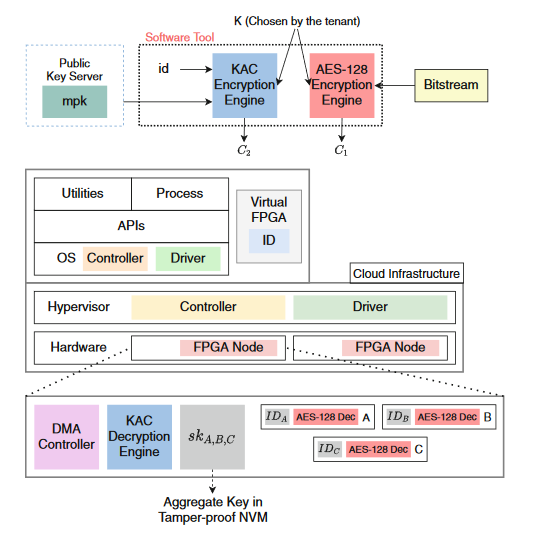
\includegraphics[width=0.6\textwidth]{bag_architecture}
    \caption[Literature Cryptosystem Implementation]{Implementation of a hybrid KAC-AES cryptosystem with one AES core per partition. \cite{bag_cryptographically_2020}}
    \label{fig:bag_architecture}
\end{figure}


In this effort's implementation, the number of AES cores is no longer linearly correlated (although perhaps necessarily proportional) to the number of partitions. Instead, it is assumed that each partition spends the majority of its time not in a state of actively being reconfigured, and therefore it is presumed feasible to share the AES cores among multiple partitions. To this end, the cores (scheduled by the EDF-based scheduler outlined in Chapter \ref{ch:edfScheduling}) are no longer statically assigned index values. Instead, these values are dynamically assigned by the scheduler as the core is assigned to a partition.

Although this mechanism does inject some additional complexity into the decryption process, it actually affords further enhanced security. By dynamically assigning the index value to the core, the capability to decrypt the AES key is no longer simply constrained to a single hardware target, but is in fact constrained to that target only during the period for which the KAC engine is specifically allocated to that partition. As the KAC engine is only decrypting a trivially small ciphertext (the AES key), it will not need to spend much time assigned to any given partition. This fact, coupled with the retention of the decrypted AES key for only as long as is needed to facilitate bitstream decryption, immensely reduces the already small vulnerable surface for bitstream compromise in the event of aggregate key leakage.